\let\negmedspace\undefined
\let\negthickspace\undefined
\documentclass[journal]{IEEEtran}
\usepackage[a5paper, margin=10mm, onecolumn]{geometry}
%\usepackage{lmodern} % Ensure lmodern is loaded for pdflatex
\usepackage{tfrupee} % Include tfrupee package

\setlength{\headheight}{1cm} % Set the height of the header box
\setlength{\headsep}{0mm}     % Set the distance between the header box and the top of the text

\usepackage{gvv-book}
\usepackage{gvv}
\usepackage{cite}
\usepackage{amsmath,amssymb,amsfonts,amsthm}
\usepackage{algorithmic}
\usepackage{graphicx}
\usepackage{textcomp}
\usepackage{xcolor}
\usepackage{txfonts}
\usepackage{listings}
\usepackage{enumitem}
\usepackage{mathtools}
\usepackage{gensymb}
\usepackage{comment}
\usepackage[breaklinks=true]{hyperref}
\usepackage{tkz-euclide} 
\usepackage{listings}
% \usepackage{gvv}                                        
\def\inputGnumericTable{}                                 
\usepackage[latin1]{inputenc}                                
\usepackage{color}                                            
\usepackage{array}                                            
\usepackage{longtable}                                       
\usepackage{calc}                                             
\usepackage{multirow}                                         
\usepackage{hhline}                                           
\usepackage{ifthen}                                           
\usepackage{lscape}
\begin{document}

\bibliographystyle{IEEEtran}
\vspace{3cm}

\title{12.489}
\author{EE25BTECH11060 - V.Namaswi}
% \maketitle
% \newpage
% \bigskip
{\let\newpage\relax\maketitle}
\renewcommand{\thefigure}{\theenumi}
\renewcommand{\thetable}{\theenumi}
\setlength{\intextsep}{10pt} % Space between text and floats
\textbf{Question}\\Matrix 
\begin{align*}
   \vec{A}= \begin{pmatrix}
        2 & 0 & 2 \\
3 & 7 & 2 \\
5 & 1 & 7
    \end{pmatrix}
,
\vec{b} =
\begin{pmatrix}
4 \\ 4 \\ 5
\end{pmatrix}
\end{align*}
are given. If vector $ \Vec{x}$ is the solution to the system of equations   $ \Vec{A}\Vec{x}=\Vec{b}$, which of the following is true for $\Vec{x}$
\begin{multicols}{2}
\begin{enumerate}[label=(\alph*)]
    \item  Solution does not exist \quad
    \item  Infinite solutions exist \quad
\item  Unique solution exists \quad
\item Five possible solutions exist

\end{enumerate} 
\end{multicols}

\textbf{Solution}\\
Given,
\begin{align}  
\vec{A} = 
\begin{pmatrix}
2 & 0 & 2 \\
3 & 7 & 2 \\
5 & 1 & 7
\end{pmatrix}
\quad
\vec{b}=
\begin{pmatrix}
4 \\ 4 \\ 5
\end{pmatrix}
\end{align}
Form the augmented matrix:
 \begin{align}
      \augvec{3}{1}{ 
      2 & 0 & 2 & 4 \\
3 & 7 & 2 & 4 \\
5 & 1 & 7 & 5   
}
 \end{align}

According to Gaussian elimination:
Replace
\[
R_2 \to R_2 - \frac{3}{2}R_1, 
\quad
R_3 \to R_3 - \frac{5}{2}R_1
\]

 \begin{align}
     \augvec{3}{1}{ 
         2 & 0 & 2 & 4 \\
0 & 7 & -1 & -2 \\
0 & 1 & 2 & -5
}
 \end{align}
Replace
\[
R_3 \to R_3 - \frac{1}{7}R_2
\]

\begin{align}
    \augvec{3}{1}{ 
       2 & 0 & 2 & 4 \\
0 & 7 & -1 & -2 \\
0 & 0 & \frac{15}{7} & \frac{-33}{7} 
}
\end{align}
Now on back-substitute:
\begin{align}
    \Vec{x}=\begin{pmatrix}
\frac{21}{5} \\
-\frac{3}{5} \\
-\frac{11}{5}
\end{pmatrix}
\end{align}
 

\[
 {\text{Hence, a unique solution exists.}}
\]
\begin{align}
\centering
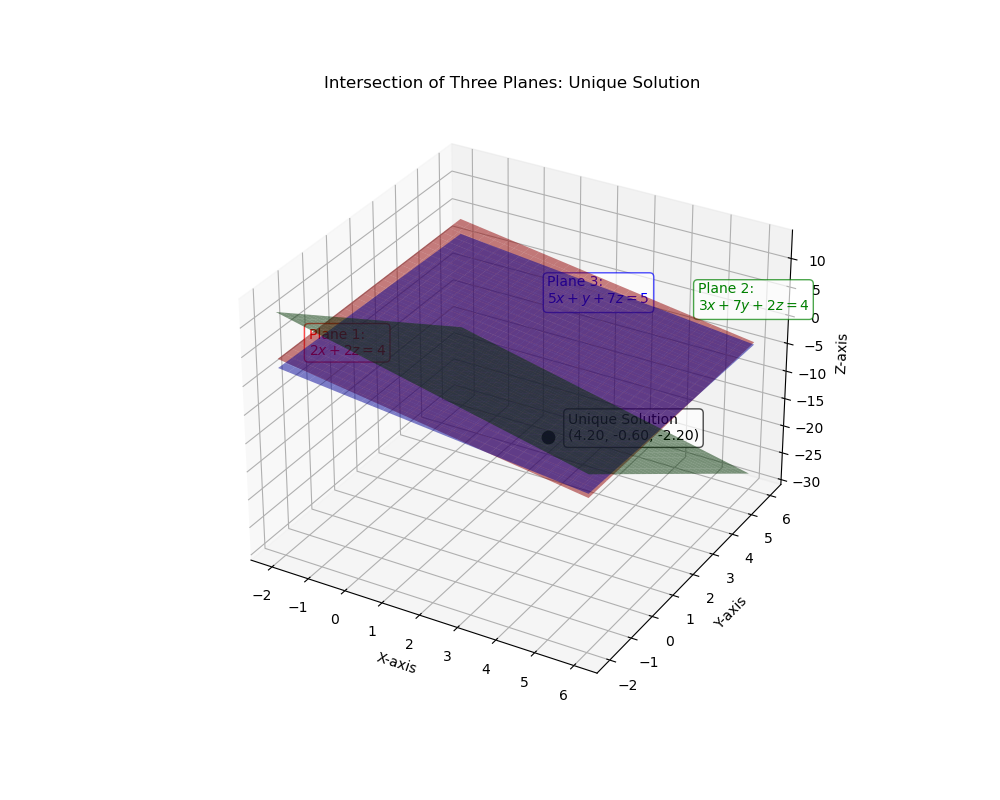
\includegraphics[width=\columnwidth, height=0.8\textheight, keepaspectratio]{figs/Figure_23.png}       
\end{align}
\end{document}